\section{Przegląd rozwiązań}
  Sieci neuronowe, dzięki swoim cechom, znalazły wiele rzeczywistych zastosowań w produktach
  przemysłowych. W tym podrozdziale skupiono się na przedstawieniu istniejących
  rozwiązań rozważanej problematyki. \textless Do zredagowania jeszcze \textgreater

  \subsection{Neural photo editing}
    W 2017 roku Andrew Brock, Theodore Lim, J.M. Ritchie and Nick Weston
    zaprezenowali Neural Photo Editor \cite{neural_photo_editor}, narzędzie
    do edytowania obrazu wyposażone w mechanizmy wykrywania kontekstu zmiany.
    Twórcy opisują swój twór następująco:

    \begin{quote}
      'An interface that leverages the power of generative neural networks to
      make large, semantically coherent changes to existing images.'

      'Interfejs wykorzystujący moc generatywnych sieci neuronowych do
      wprowadzania dużych, semantycznie spójnych zmian w istniejących obrazach.'
    \end{quote}

    Użytkowanie wygląda następująco: użytkownik pędzlem o określonym kolorze i
    rozmiarze maluje na wybranym obrazie, jednak zamiast zmieniać wartości
    pojedynczych pikseli, interfejs odczytuje konteks edycji i wprowadza zmiany
    semantyczne w kontekście żądanej zmiany koloru. Efekt działania interfejsu
    został przedstawiony na Rysunku \ref{fig:npe}.

    \begin{figure}[h]
      \centering
      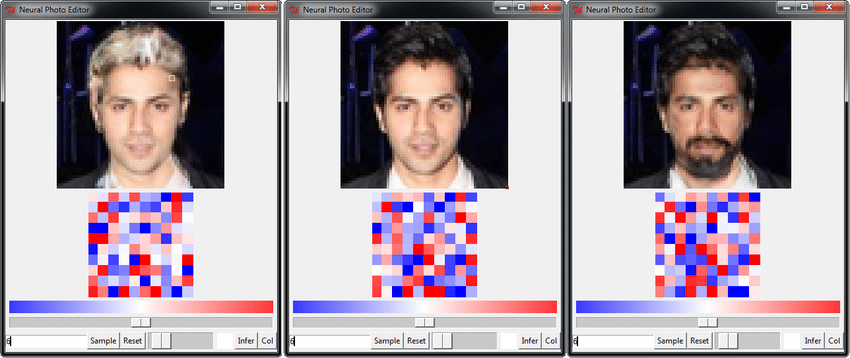
\includegraphics[width=4in]{NPE}
      \caption{Efekt działania Neural Photo Editor.}
      \label{fig:npe}
    \end{figure}

    Skuteczność NPE (Neural Photo Editor) polega na zastosowaniu IAN
    (ang. Introspective Adversarial Network), czyli sieci złożonej z połączonych
    VAE (ang. Variational Autoencoder) oraz GAN, w taki sposób, żę dekodująca
    sieć autoenkodera jest używana jako sieć generująca w GAN.
    Poprzez przechwytywanie przez model dalekosiężnych zależności, wykorzystanie
    bloku obliczeniowego bazującego na rozszerzonych splotach o
    współdzielonych wagach oraz dzięki zastosowaniu ulepszonej generalizacji,
    udało się osiągnąć dokładną rekonstrukcje obrazu bez strat na jakości detali.


  \subsection{Colorful image colorization}

    Wraz z rozwojem sieci neuronowych, rosło zainteresowanie możliwościami zastosowania
    ich do kolorowania czarno-białych obrazów. Jedno z dostępnych rozwiązań tego
    zagadnienia zostało przedstawione przez grupę pracowników Uniwersytetu w
    Berkeley \cite{colorful_image_colorization}. Zamiarem ich pracy było stworzenie
    modelu, który niekoniecznie odtwarza oryginalne barwy obrazu, ale generuje
    barwy prawdopodbne, zdolne przekonać ludzkiego obserwatora o autentyczności
    obrazu. Uzyskane rezultaty zostały przedstawione na
    Rysunku \ref{fig:colorful_image_colorization}.

    \begin{figure}[h]
      \centering
      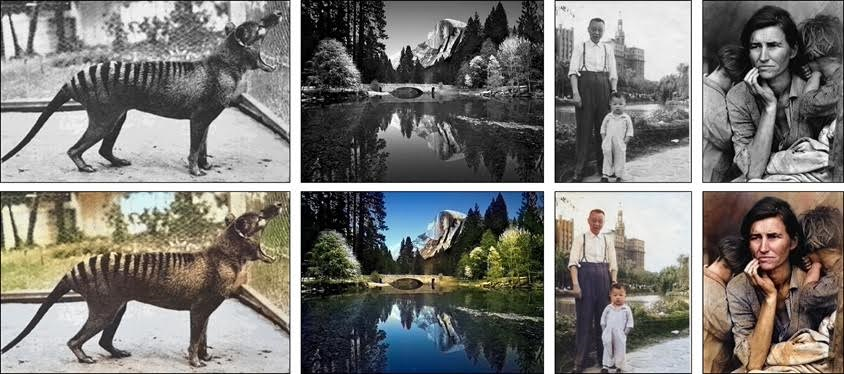
\includegraphics[width=4in]{image_colorization}
      \caption{Efekt kolorowanie czarno-białych zdjęć przez wytrenowany model.}
      \label{fig:colorful_image_colorization}
    \end{figure}

    Wykorzystany model składa się z wielu warst CNN, w których skład wchodzą
    warsta filtrów konwolucyjnych, warsta ReLU (ang. Rectified
    Linear Unit) oraz warstwa BatchNorm (ang. Batch normalization).
    Aby zapobiec utracie informacji przestrzennych, sieć nie posiada warst łączących.
    Istotny był także sposób
    przygotowania zbioru danych do trenowania modelu. Obrazy ze zbioru uczącego
    były wpier konwertowane do modelu YUV, a następnie kanał Y był podawany na
    wejście modelu, warstwy UV pełniły funkcję pożądnej odpowiedzi w uczeniu
    nadzorowanym.

    Ważnym aspktem zbadanym w artykule było także dobranie odpowiedniej
    funkcji kosztu. Nieodpowiedni wybór skutkował desaturacją kolorowanych
    obrazów, jedną z potencjalnych przyczyn tego zjawiska może być tendencja
    sieci do tworzenia bardziej konserwatwynych odpowiedzi. Aby zniwelować ten
    efekt w modelu została zastosowana specjalna technika modyfikacji
    funkcji kosztu. Polega ona na przewidywaniu dystrybucji możliwych kolorów
    dla każdego piksela i zmienianiu kosztu dla modelu, w celu wyróżnienia rzadko
    spotykanych kolorów.

  \subsection{Image Style Transfer Using Convolutional Neural Networks}
    W roku 2016 został przedstawiony światu A Neural Algorithm of Artistic Style
    \cite{image_style_transfer}. Wprowadzał on przełom w dziedzinie przenoszenia
    stylu jednego obrazu na inny, a jego suckes opierał się na właściwym wykorzystaniu
    konwolucyjnych sieci neuronowych. Podstawą tego sukcesu było odkrycie przez
    Leona A. Gatys oraz jego współpracowników, że w CNN reprezentacja treści
    obrazu oraz jego stylu jest rozłączna. Umożliwia to wydobycie stylu
    przetwarzanego obrazu oraz połączenie go z treścią innego obrazu, czego
    dokonuje właśnie A Neural Algorithm of Artistic Style. Rezultaty takich
    operacji można zaobserwować na Rysunku \ref{fig:image_style_transfer}

    \begin{figure}[h]
      \centering
      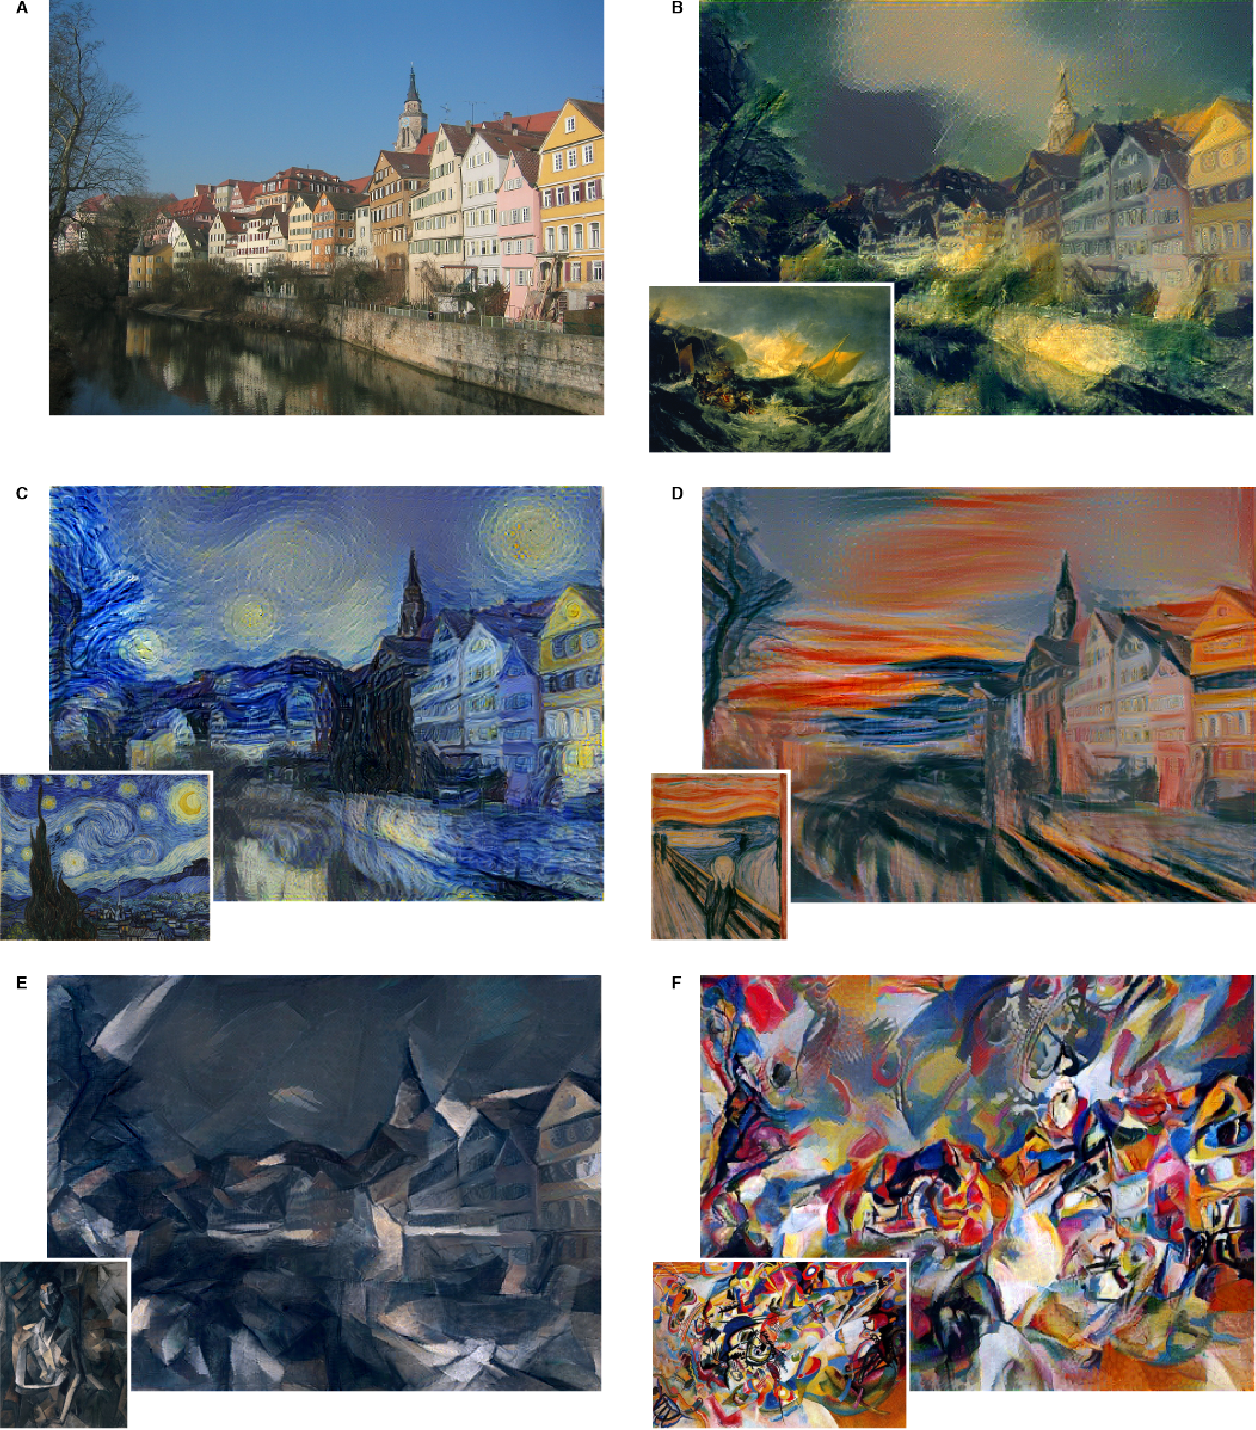
\includegraphics[width=4in]{image_style_transfer}
      \caption{Obrazy będące kombinacją treści zdjęcia ze stylami kilku znanych dzieł sztuki.}
      \label{fig:image_style_transfer}
    \end{figure}

    Do zbudowania modelu zostały użyte warsty konwolucyjne oraz łączące z
    architektury VGG-Network \cite{vgg_network}, która została wytrenowana pod
    kątem rozpoznawanie obiektów i określania ich położenia. Dzięki temu sieć
    przetwarzając obraz tworzy jego reprezentację, która wraz z
    kolejnymi warstwami, przedstawia coraz wyraźniejszą informację o obiektach,
    a niekoniecznie o dokładnym wyglądzie obrazu.
    W modelu nie została użyta ani jedna warstwa gęsta, dzięki czemu na wyjściu
    możliwe jest otrzymanie dwuwymiarowego obrazu.
    Dla lepszej syntezy obrazów, w warstwach
    łączących zastosowano próbkowanie wartością średnią zamiast maksymalną.
    Takie zabiegi umożliwiają wyliczenie reprezentacji stylu z korelacji
    pomiędzy różnymi cechami w różnych warstwach konwolucyjnych.

    Cały proces renderowania polega na odpowiednim zapisaniu w modelu treści
    oraz stylu obrazów otrzymanych przez wcześniejsze podanie na model tychże
    obrazów. Wpier obraz, z którego pobierany jest styl, jest podawany na
    wejście sieci oraz przeliczany, reprezentacja stylu wyselekcjonowana z
    właściwych warst jest przechowywana, obraz z treścią jest poddawany temu samemu
    procesowi, ale reprezentacja treści jest wyciągana z ostatnich
    warst konwolucyjnych.
    W celu uzyskania fuzji obrazów, zapisane reprezentacje treści i stylu są
    zapisywane w tych warstwach modelu skąd zostały odczytane, a następnie na wejście
    podawany jest obraz składający się z losowego szumu białego.
    Następnie poprzez iteracyjną minimalizację funckji kosztu, obraz wejściowy jest modyfikowany, co w rezultacie końcowym doprowadza do nałożenia zapisanego
    stylu na wczytaną treść.



  \subsection{Transforming photos to comics using convolutional neural networks}

  \subsection{Face App}
